\documentclass[printbox]{BHCexam}
\biaoti{第一学期期末考试}
\fubiaoti{高一数学试卷}


\begin{document}
\maketitle
%\mininotice
\notice
\begin{questions}

%选择题
\xuanze
\question ~$\tan 300^{\circ}$~的值为\xx.
\onech{$\dfrac{\sqrt{3}}{3}$}{$-\dfrac{\sqrt{3}}{3}$}{$\sqrt{3}$}{$-\sqrt{3}$}
\question 已知全集~$U=R$~,集合~$A=\{ x|~1<x<3 \}~,B=\{ x|~x>2 \}$~,则~$A\cap \complement _U B=$~\xx.
\onech{$\{x|~1<x\leq 2 \}$}{$\{x|~2<x<3 \}$}{$\{x|~1<x<2 \}$}{$\{x|~x\leq 2 \}$}
\question 已知角~$\alpha$~终边上有一点~$P(3,-4)$~,则~$\cos \alpha$~的值是\xx.
\onech{$-\dfrac{4}{5}$}{$\dfrac{3}{5}$}{$\pm \dfrac{3}{5}$}{$\pm \dfrac{4}{5}$}
\question 下列函数中,既是奇函数又是偶函数的为\xx.
\onech{$y=x+1$}{$y=-x^2$}{$y=\dfrac{1}{x}$}{$y=x \abs{x}$}
\question 若~$O$~为平面内任一点且~$(\overrightarrow{OB}+\overrightarrow{OC}-2~\overrightarrow{OA})\cdot (\overrightarrow{AB}-\overrightarrow{AC})=0$~,则~$\triangle ABC$~是\xx.
\twoch{直角三角形或等腰三角形}{等腰直角三角形}{等腰三角形但不一定是直角三角形}{直角三角形但不一定是等腰三角形}
\question 函数~$f(x)=e^x+x-2$~的零点所在的区间是\xx.
\onech{$(0,\dfrac{1}{2})$}{$(\dfrac{1}{2},1)$}{$(1,2)$}{$(2,3)$}
\question 已知~$a=0.2^{0.3},b=\log_{0.2} 3,c=\log_{0.2} 4$~,则\xx.
\onech{$b>c>a$}{$a>c>b$}{$a>b>c$}{$c>b>a$}
\question 某地西红柿从~$2$~月~$1$~日起开始上市,通过市场调查,得到西红柿种植成本~$Q$~(单位:元/$10^2 kg$)与上市时间~$t$~(单位:天)的数据如下表:
\begin{center}
\begin{tabular}{|c|c|c|c|}
\hline
~~~~~时间~~~$t$~~~~~&$~~~~50~~~~$&$~~~~110~~~~$&$~~~~250~~~~$\\
\hline
~~~~~种植成本~~~$Q$~~~~~&$~~~~150~~~~$&$~~~~108~~~~$&$~~~~150~~~~$\\
\hline
\end{tabular}
\end{center}
根据上表数据,对于下列四种函数类型,你觉得哪种函数类型描述西红柿种植成本~$Q$~与上市时间~$t$~的变化关系最合适?\xx.
\onech{$Q=at+b$}{$Q=at^2+bt+c$}{$Q=a\cdot b^t$}{$Q=a\cdot \log_b t$}
\question {\kaishu (选做一)} 已知~$f(x)=sin {2x}$~要得到函数~$y=cos {2x}$~的图象,只需将函数~$y=f(x)$~的图象\xx.
\twoch{向左平移~$\dfrac{\pi}{2}$~个单位长度}{向右平移~$\dfrac{\pi}{2}$~个单位长度}
{向左平移~$\dfrac{\pi}{4}$~个单位长度}{向右平移~$\dfrac{\pi}{4}$~个单位长度}
\begin{minipage}[b]{0.7\linewidth}
{\kaishu(选做二)} 已知函数~$f(x)=A sin(\omega x+\varphi)$~(其中~$A>0,\abs{\varphi}<\dfrac{\pi}{2}$~)的部分图象如下图所示,为了得到~$g(x)=sin {2 x}$~的图象,则只需将~$f(x)$~的图象\xx.
\twoch{向左平移~$\dfrac{\pi}{12}$~个单位长度}{向右平移~$\dfrac{\pi}{12}$~个单位长度}{向左平移~$\dfrac{\pi}{6}$~个单位长度}{向右平移~$\dfrac{\pi}{6}$~个单位长度}
\end{minipage}
\hfill
\begin{minipage}[b]{0.3\linewidth}
\begin{flushright}
\begin{tikzpicture}[scale=0.9]
\coordinate[label=below right:\small $O$] (O) at(0,0);
\coordinate[label=above :\small $\dfrac{\pi}{3}$] (t1) at(pi/3,0);
\coordinate[label=above :\small $\dfrac{7\pi}{12}$] (t2) at(7*pi/12,0);
\draw[densely dashed](0,1)--(pi/12,1);
\draw[->,>=latex](-pi/2,0)--(pi,0)node[below](x) {$x$};
\draw[->,>=latex](0,-1.5)--(0,1.5)node[right](y) {\small $y$};
\draw [domain=-pi/6:5*pi/6,samples=1000] plot(\x,{sin((2*(\x)+pi/3) r)});
\draw[densely dashed](0,-1)--(7*pi/12,-1)--(7*pi/12,0);
\node[left](pi) at(0,-1) {\small $-1$};
\node[left](pi) at(0,1) {\small $1$};
\end{tikzpicture}
\end{flushright}
\end{minipage}
\question {\kaishu (选做一)}李明放学回家的路上,开始和同学边走边讨论问题,走得比较慢;然后他们索性停下来将问题彻底解决,最后他快速地回到了家。下列图象中与这一过程吻合最好的是\xx.\\
\begin{center}
\begin{tikzpicture}
\draw[->,>=latex](0,0)--(2,0)node[below](x){时间};
\draw[->,>=latex](0,0)--(0,1.5)node[right](y){离家的距离};
\draw(0,0)--(0.2,0.8)--(0.7,0.8)--(1.6,0);
\coordinate[label=below:$(\mathrm{A})$] (A) at(1,-0.4);
\begin{scope}[xshift=1cm]
\draw[->,>=latex](3,0)--(5,0)node[below](x){时间};
\draw[->,>=latex](3,0)--(3,1.5)node[right](y){离家的距离};
\draw(3,0)--(4,0.8)--(4.4,0.8)--(4.6,0);
\coordinate[label=below:$(\mathrm{B})$] (B) at(4,-0.4);
\end{scope}
\begin{scope}[xshift=2cm]
\draw[->,>=latex](6,0)--(8,0)node[below](x){时间};
\draw[->,>=latex](6,0)--(6,1.5)node[right](y){离家的距离};
\draw(6,1)--(6.2,0.3)--(6.8,0.3)--(7.6,0);
\coordinate[label=below:$(\mathrm{C})$] (C) at(7,-0.4);
\end{scope}
\begin{scope}[xshift=3cm]
\draw[->,>=latex](9,0)--(11,0)node[below](x){时间};
\draw[->,>=latex](9,0)--(9,1.5)node[right](y){离家的距离};
\draw(9,1)--(10,0.6)--(10.4,0.6)--(10.6,0);
\coordinate[label=below:$(\mathrm{D})$] (D) at(10,-0.4);
\end{scope}
\end{tikzpicture}	
\end{center} 

{\kaishu (选做二)}函数~$y=\dfrac{x ln {\abs{x}}}{\abs{x}}$~的图象可能是\xx.

\begin{center}
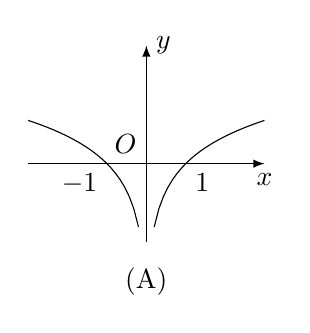
\begin{tikzpicture}[scale=0.5]
\draw[->,>=latex](-3,0)--(3,0)node[below](x){$x$};
\draw[->,>=latex](0,-2)--(0,3)node[right](y){$y$};
\coordinate[label=above left:$O$](O) at(0,0);
\draw[domain=0.2:3]plot(\x,{ln \x});
\draw[domain=-3:-0.2]plot(\x,{ln (-\x )});
\node[below left] at (-1,0){$-1$};
\node[below right] at (1,0){$1$};
\coordinate[label=below:$(\mathrm{A})$] (A) at(0,-2.4);
\end{tikzpicture}
\qquad \qquad
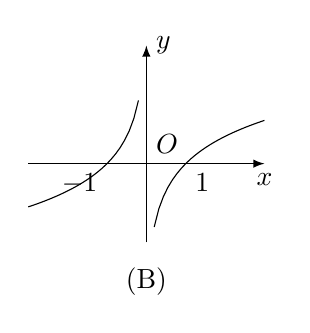
\begin{tikzpicture}[scale=0.5]
\draw[->,>=latex](3,0)--(9,0)node[below](x){$x$};
\draw[->,>=latex](6,-2)--(6,3)node[right](y){$y$};
\coordinate[label=above right:$O$](O) at(6,0);
\draw[domain=6.2:9]plot(\x,{ln (\x-6)});
\draw[domain=3:5.8]plot(\x,{-(ln (6-\x))});
\node[below left] at (5,0){$-1$};
\node[below right] at (7,0){$1$};
\coordinate[label=below:$(\mathrm{B})$] (B) at(6,-2.4);
\end{tikzpicture} \\
\begin{tikzpicture}[scale=0.5]
\draw[->,>=latex](-3,0)--(3,0)node[below](x){$x$};
\draw[->,>=latex](0,-2)--(0,3)node[right](y){$y$};
\coordinate[label=below left:$O$](O) at(0,0);
\draw[domain=0.3:3]plot(\x,{-(ln \x )});
\draw[domain=-3:-0.3]plot(\x,{-(ln (-\x ))});
\node[below left] at (-1,0){$-1$};
\node[below right] at (1,0){$1$};
\coordinate[label=below:$(\mathrm{C})$] (C) at(0,-2.4);
\end{tikzpicture}
\qquad \qquad
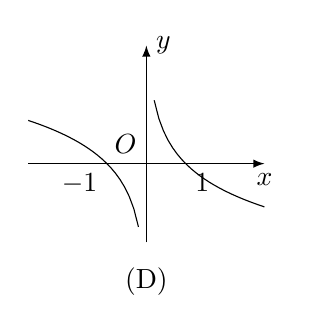
\begin{tikzpicture}[scale=0.5]
\draw[->,>=latex](3,0)--(9,0)node[below](x){$x$};
\draw[->,>=latex](6,-2)--(6,3)node[right](y){$y$};
\coordinate[label=above left:$O$](O) at(6,0);
\draw[domain=6.2:9]plot(\x,{-(ln (\x-6))});
\draw[domain=3:5.8]plot(\x,{ln (6-\x)});
\node[below left] at (5,0){$-1$};
\node[below right] at (7,0){$1$};
\coordinate[label=below:$(\mathrm{D})$] (D) at(6,-2.4);
\end{tikzpicture}	
\end{center} 
%填空题
\tiankong
\question 函数~$y=log_a {(x-2)-1}$~($a>0$~且~$a\neq 1$)的图象恒过的定点的坐标是\mtk{}.
\question 若~$\vec{a}=(1,2),\vec{b}=(-1,0)$~,则~$\vec{a}$~在~$\vec{b}$~方向上的投影等于\mtk{}.
\question 已知~$a\in (\dfrac{\pi}{2},\pi),sin \alpha=\dfrac{\sqrt{5}}{5}$~,则~$tan (\alpha-\dfrac{\pi}{4})=$~\mtk{}.
\question {\kaishu (选做一)}已知:~$f(x)= \begin{cases}
2^ {x-2}~~~~~~~~~(x\leq 2)\\
log_2 (x-1)~~(x>2) 
\end{cases}$,则~$f[f(5)]$~等于\mtk{}.\\
{\kaishu (选做二)}已知函数~$f(x)= \begin{cases}
-x^2-4x,x\geq 0\\
x^2-4x,x<0
\end{cases}$,若~$f(a-2)+f(a)>0$~,则实数~$a$~的取值范围是\mtk{}.

%解答题
\jianda
\question (本题满分12分)\\
已知~$cos \alpha =\dfrac{1}{7},cos(\alpha+\beta)=-\dfrac{11}{14}$~,且~$\alpha,\beta\in (0,\dfrac{\pi}{2})$~,求~$cos\beta$~的值.
\vspace{7cm}
\question (本题满分12分)\\
{\kaishu (选做一)}已知函数~$f(x)=log_4 (3^x-1)$.
\begin{parts}
\part 求~$f(x)$~的定义域;
\part 求~$f(1)+f(2)$~的值.
\end{parts}
{\kaishu (选做二)}已知函数~$f(x)=log_a (a^x-1)$~($a>0$~且~$a\neq 1$)~.
\begin{parts}
\part 求函数~$f(x)$~的定义域;
\part 若~$f(x)>1$~,求~$x$~的取值范围.
\end{parts}
\vspace{8cm}
\question (本题满分12分)\\
已知~$\vec{a}=(\sqrt{3} sin x,cos x),\vec{b}=(cos x,cos x),x\in R$~,函数~$f(x)=2\,\vec{a}\cdot \vec{b}-1$~.\\%
(1) 求~$f(x)$~的最小正周期及其单调递减区间;\\
{\kaishu (选做一)}(2) 求~$f(x)$~的最大值和最小值及取得最大值、最小值时~$x$~的值。\\
{\kaishu (选做二)}(2) 求~$f(x)$~在区间~$\left[ -\dfrac{\pi}{6},\dfrac{\pi}{4} \right]$~上的最大值和最小值及取得最大、最小值时~$x$~的值。
\vspace{7cm}
\question (本题满分13分)\\
{\kaishu (选做一)}已知函数~$f(x)=2^x-2^{-x}$~.
\begin{parts}
\part 求函数~$f(x)$~的零点;
\part 判断函数~$f(x)$~的奇偶性;
\part 证明函数~$f(x)$~在~$R$~上是增函数.
\end{parts}
{\kaishu (选做二)}已知函数~$f(x)=2^x+\lambda \cdot 2^{-x}~(x\in R)$~.
\begin{parts}
\part 当~$\lambda =-1$~时,求函数~$f(x)$~的零点;
\part 若函数~$f(x)$~为偶函数,求实数~$\lambda$~的值,判断此时函数~$f(x)$~在~$[0,+\infty)$~上的单调性,并证明;
\part 当~$x\in [0,2]$~时,$f(x)\leq 2^{x+1}-3$~恒成立,求~$\lambda$~的取值范围。
\end{parts}
\begin{solution}
\begin{parts}
\part 

\part 
\part $f(x)\leq 2^{x+1}-3$~可得~$2^x+\lambda \cdot 2^{-x}\leq 2^{x+1}-3$  \\
$\lambda \leq 2\cdot (2^x)^2-3\cdot 2^x-(2^x)^2$,即~$\lambda \leq (2^x)^2-3\cdot 2^x$ \\
令~$t=2^x$~,当~$x\in [0,2]$~时,~$t\in [1,4]$ \\
当~$x\in [0,2]$~时,$f(x)\leq 2^{x+1}-3$~恒成立即转化为当~$t\in [1,4]$~时,$\lambda \leq t^2-3t$~恒成立。\\
当~$t\in [1,4]$~时,$t^2-3t\in [-\dfrac{9}{4},4]$ \\
$\therefore \lambda \leq -\dfrac{9}{4}$   ~~~~~~~~~~~~~~~~~~~~~~~~~~~~~~~~~$\cdots  \cdots  \cdots  \cdots  \cdots  \cdots$~~$13$分
\end{parts}
\end{solution}
\end{questions}
\end{document}
